%%%%%%%%%%%%%%%%%%%%%%%%%%%%%%%%%%%%%%%%%
% Jacobs Portrait Poster
% LaTeX Template
% Version 1.0 (31/08/2015)
% (Based on Version 1.0 (29/03/13) of the landscape template
%
% Created by:
% Computational Physics and Biophysics Group, Jacobs University
% https://teamwork.jacobs-university.de:8443/confluence/display/CoPandBiG/LaTeX+Poster
% 
% Further modified by:
% Nathaniel Johnston (nathaniel@njohnston.ca)
%
% Portrait version by:
% John Hammersley
%
% The landscape version of this template was downloaded from:
% http://www.LaTeXTemplates.com
%
% License:
% CC BY-NC-SA 3.0 (http://creativecommons.org/licenses/by-nc-sa/3.0/)
%
%%%%%%%%%%%%%%%%%%%%%%%%%%%%%%%%%%%%%%%%%

%----------------------------------------------------------------------------------------
%	PACKAGES AND OTHER DOCUMENT CONFIGURATIONS
%----------------------------------------------------------------------------------------


\documentclass[final]{beamer}

\usepackage[scale=1.2]{beamerposter} % Use the beamerposter package for laying out the poster

%\usepackage[scale=0.78,size=a1]{beamerposter}
%\setlength{\paperwidth}{33.1in}
%\setlength{\paperheight}{23.4in}

\usetheme{confposter} % Use the confposter theme supplied with this template

\setbeamercolor{block title}{fg=ngreen,bg=white} % Colors of the block titles
\setbeamercolor{block body}{fg=black,bg=white} % Colors of the body of blocks
\setbeamercolor{block alerted title}{fg=white,bg=dblue!70} % Colors of the highlighted block titles
\setbeamercolor{block alerted body}{fg=black,bg=dblue!10} % Colors of the body of highlighted blocks
% Many more colors are available for use in beamerthemeconfposter.sty

%-----------------------------------------------------------
% Define the column widths and overall poster size
% To set effective sepwid, onecolwid and twocolwid values, first choose how many columns you want and how much separation you want between columns
% In this template, the separation width chosen is 0.024 of the paper width and a 4-column layout
% onecolwid should therefore be (1-(# of columns+1)*sepwid)/# of columns e.g. (1-(4+1)*0.024)/4 = 0.22
% Set twocolwid to be (2*onecolwid)+sepwid = 0.464
% Set threecolwid to be (3*onecolwid)+2*sepwid = 0.708

\newlength{\sepwid}
\newlength{\onecolwid}
\newlength{\twocolwid}
\newlength{\threecolwid}
\setlength{\paperwidth}{36in} % A0 width: 46.8in
\setlength{\paperheight}{48in} % A0 height: 33.1in
\setlength{\sepwid}{0.024\paperwidth} % Separation width (white space) between columns
\setlength{\onecolwid}{0.22\paperwidth} % Width of one column
\setlength{\twocolwid}{0.464\paperwidth} % Width of two columns
\setlength{\threecolwid}{0.708\paperwidth} % Width of three columns
\setlength{\topmargin}{-0.5in} % Reduce the top margin size
%-----------------------------------------------------------

\usepackage{graphicx}  % Required for including images

\usepackage{booktabs} % Top and bottom rules for tables
%-----------------------------------------------------------
% Mathematics packages
\usepackage{amsthm, amsmath, amssymb, amsfonts, nicefrac, mathpazo} 
\newtheorem{mydef}{Definition}
\usepackage{diagbox} %Diagonal boxes in tables
% Easier to call Naturals, Integers and so on.
\newcommand{\N}{\mathbb{N}}
\newcommand{\Z}{\mathbb{Z}}
\newcommand{\Q}{\mathbb{Q}}
\newcommand{\C}{\mathbb{C}}
\newcommand{\ind}{1\hspace{-2.1mm}{1}} %Indicator Function
\newcommand{\I}{\mathtt{i}}
\newcommand{\EE}{\mathbb{E}}
\newcommand{\RR}{\mathbb{R}}
\newcommand{\PP}{\mathbb{P}}
\newcommand{\D}{\mathrm{d}}
\newcommand{\Xe}{X^{\varepsilon}}
\newcommand{\E}{\mathrm{e}}
\newcommand{\Tr}{\mathrm{Tr}}
\newcommand{\HH}{\mathrm{H}}
\newcommand{\sgn}{\mathrm{sgn}}
\newcommand{\atanh}{\mathrm{arctanh}}
\newcommand{\Lagr}{\mathcal{L}}
\def\equalDistrib{\,{\buildrel \Delta \over =}\,}
\DeclareMathOperator*{\argmin}{argmin}
\DeclareMathOperator*{\argmax}{argmax} 
% Writing Algorithms
\usepackage[]{algpseudocode}
%-----------------------------------------------------------


%----------------------------------------------------------------------------------------
%	TITLE SECTION 
%----------------------------------------------------------------------------------------

\title{Study of an Annular Model of Planetary Convection} % Poster title

\author{Yadu \emph{Bhageria}} % Author(s)

\institute{M4N10: Computational Partial Differential Equations, Department of Mathematics, Imperial College London} % Institution(s)
%\institute{} % Institution(s)

%----------------------------------------------------------------------------------------

\begin{document}

\addtobeamertemplate{block end}{}{\vspace*{1ex}} % White space under blocks
\addtobeamertemplate{block alerted end}{}{\vspace*{2ex}} % White space under highlighted (alert) blocks

\setlength{\belowcaptionskip}{2ex} % White space under figures
\setlength\belowdisplayshortskip{2ex} % White space under equations

\begin{frame}[t] % The whole poster is enclosed in one beamer frame

\begin{columns}[t] % The whole poster consists of three major columns, the second of which is split into two columns twice - the [t] option aligns each column's content to the top

\begin{column}{\sepwid}\end{column} % Empty spacer column

\begin{column}{1\onecolwid} % The first column

%----------------------------------------------------------------------------------------
%	OBJECTIVES
%----------------------------------------------------------------------------------------

\begin{alertblock}{Objective}

To study the behaviour of thermal convection in an annulus. 

This was done by combining the solutions of two sub-problems:

\begin{enumerate}
	\item Solving the Advection-Diffusion equation for a scalar quantity given the velocity field and Dirichlet BCs.
	\item Solving the vorticity equation and consequently deriving the stream function, $\psi$, to compute the velocity field, \textbf{u}, for Dirichlet BCs.
\end{enumerate}

\end{alertblock}

%----------------------------------------------------------------------------------------
%	INTRODUCTION
%----------------------------------------------------------------------------------------

\begin{block}{Introduction}

Thermal convection occurs because of fluids undergoing thermal expansion. This leads to changes in buoyancy within a fluid with a non-uniform temperature field that ultimately leads to convection under the influence of gravity. An everyday example of this phenomena is how convection currents develop in water boiling on a pan heated from below (Figure \ref{fig:convection}).

 An annulus is a plane figure consisting of the area between a pair of concentric circles. As such it can be used as a simplified description of the volume between 3D spheres. 
 
Thus thermal convection in an annulus is an interesting problem applicable in many situations. One example would be the flow of molten iron in the Earth's outer core (Figure \ref{fig:convection}). This in turn even affects the magnetic field of the earth \cite{MoltenCore}.

\end{block}

%------------------------------------------------

\begin{figure}
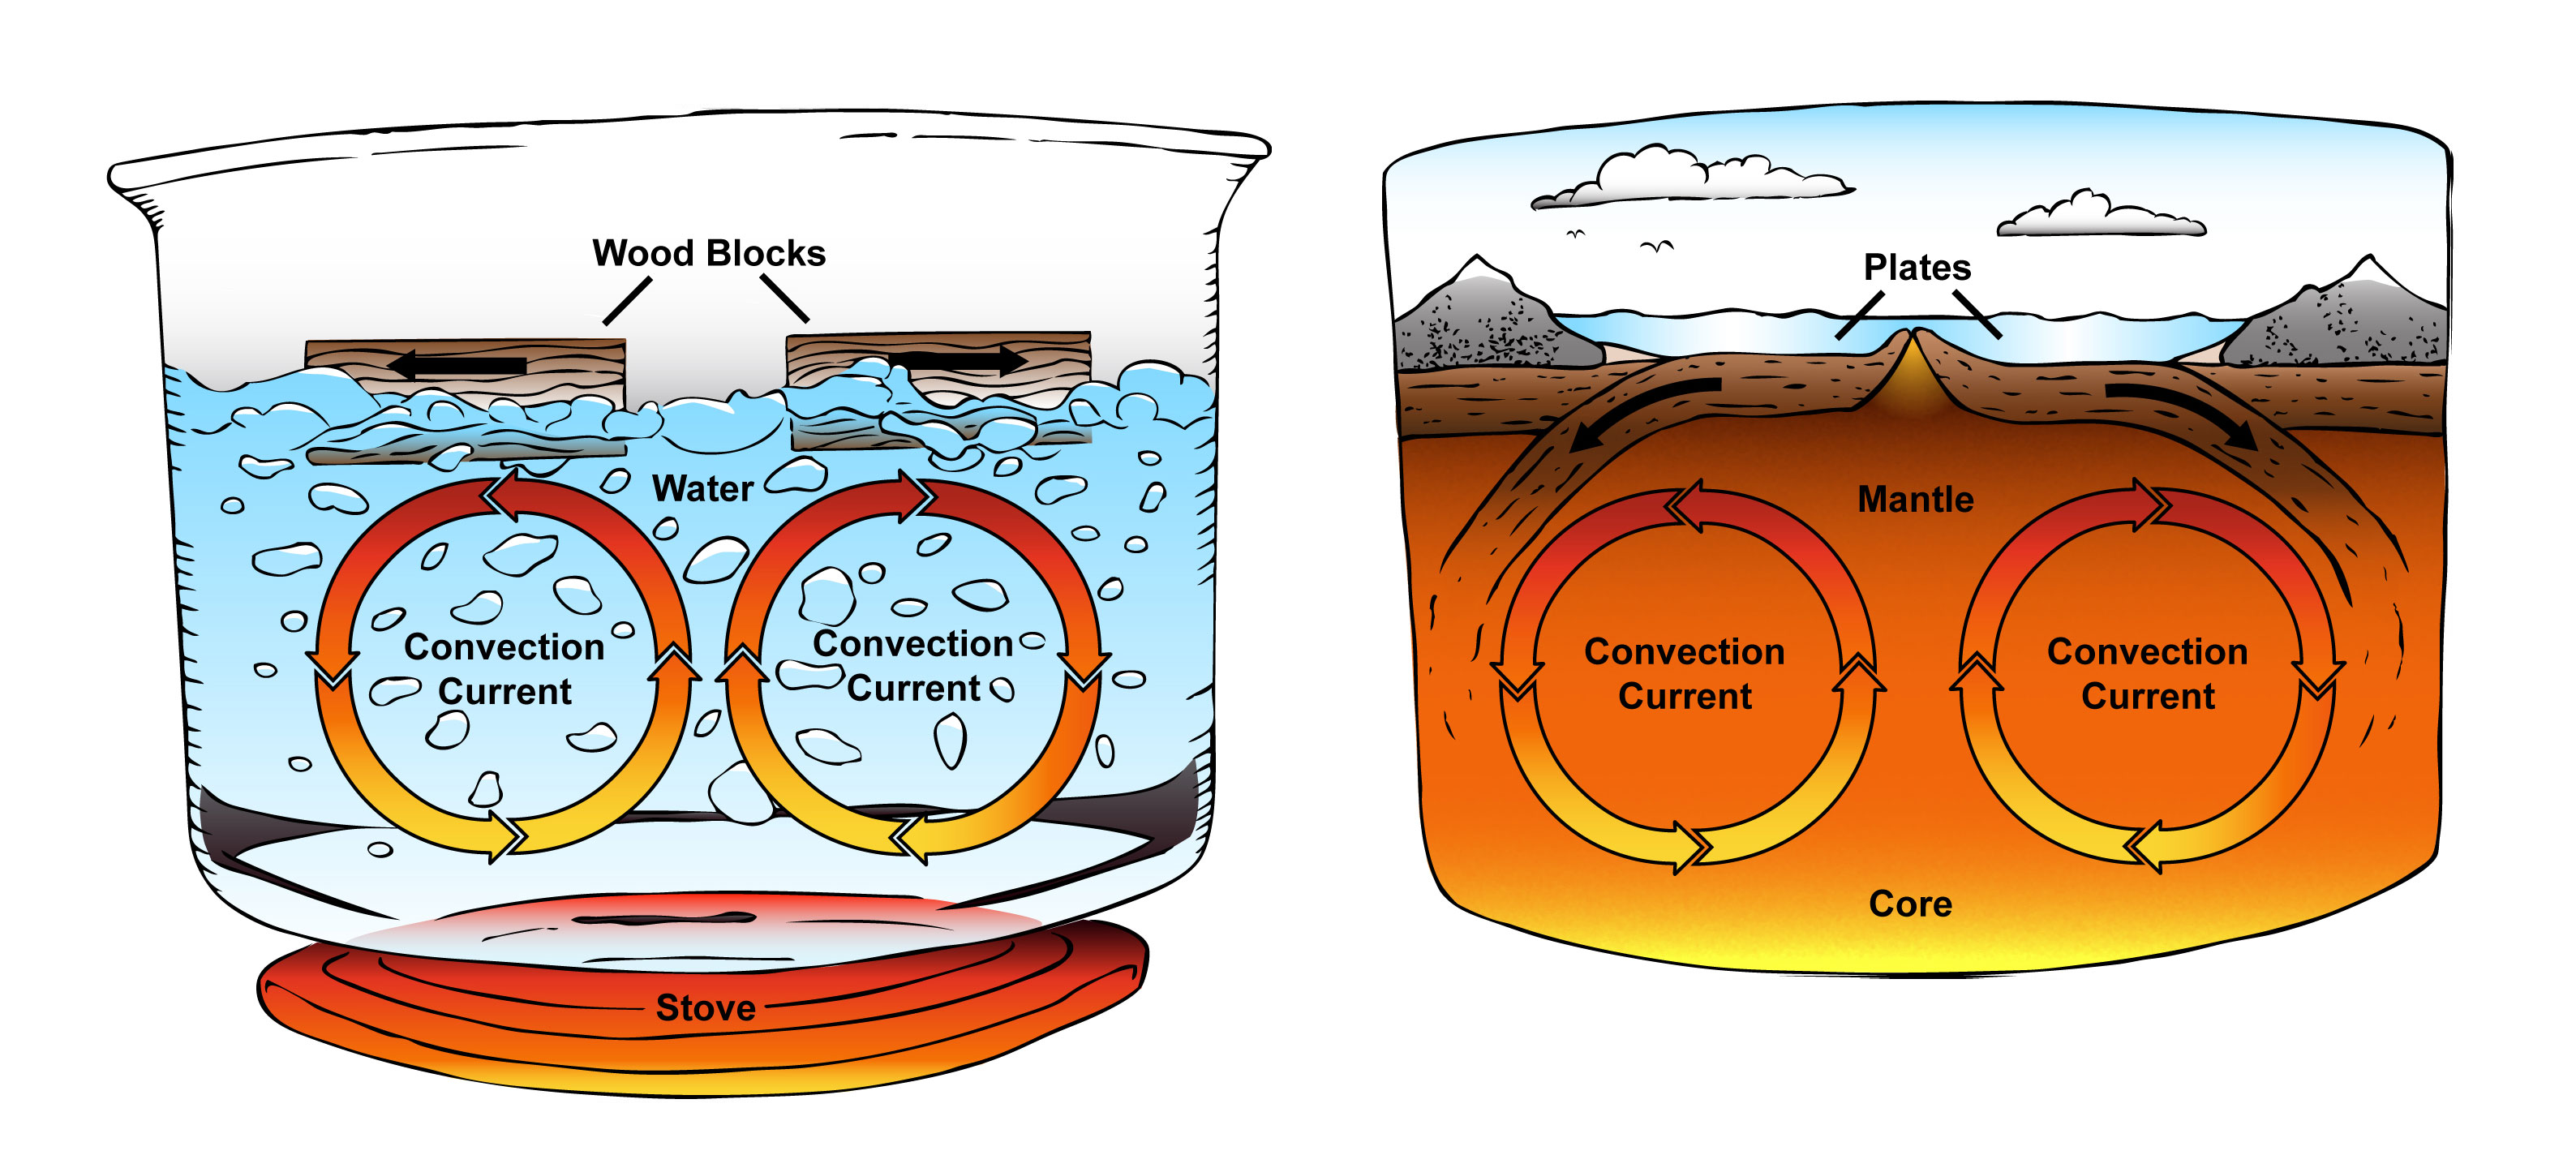
\includegraphics[width= 1.1\linewidth]{fig_waterBoiling.jpg}
\caption{Motion of liquid iron in the Earth's outer core compared to boiling water \cite{ConvectionImage}}
\label{fig:convection}
\end{figure}

%----------------------------------------------------------------------------------------
%	ESSENTIAL VOCAB
%----------------------------------------------------------------------------------------

\setbeamercolor{block alerted title}{fg=black,bg=norange} % Change the alert block title colors
\setbeamercolor{block alerted body}{fg=black,bg=white} % Change the alert block body colors

\begin{alertblock}{Useful Definitions}
{\small
\begin{itemize}
\item $R_a$: The Rayleigh number is a measure of the thermal driving force.
\item $P_r$: The Prandtl number is the ratio of the fluid kinematic viscosity to the thermal diffusivity
\item $\kappa$: The ratio between the impact of advection to diffusion for the temperature being convected
\item BCs: Boundary Conditions
\end{itemize}
}
\end{alertblock}

%----------------------------------------------------------------------------------------

\end{column} % End of the first column
%%%%%%%%%%%%%%%%%%%%%%%%%%%%%%%%%%%%%%%%%%%%%%%%%%%%%%%%%%%%%%%%%%%%%%%%%%%%%%%%
%%%%%%%%%%%%%%%%%%%%%%%%%%%%%%%%%%%%%%%%%%%%%%%%%%%%%%%%%%%%%%%%%%%%%%%%%%%%%%%%
%%%%%%%%%%%%%%%%%%%%%%%%%%%%%%%%%%%%%%%%%%%%%%%%%%%%%%%%%%%%%%%%%%%%%%%%%%%%%%%%
\begin{column}{\sepwid}\end{column} % Empty spacer column

\begin{column}{\twocolwid} % Begin a column which is two columns wide (column 2)

\begin{columns}[t,totalwidth=\twocolwid] % Split up the two columns wide column

\begin{column}{\onecolwid}\vspace{-.6in} % The first column within column 2 (column 2.1)

%----------------------------------------------------------------------------------------
%	MATERIALS
%----------------------------------------------------------------------------------------

\begin{block}{Governing Equations}

The non-dimensionalized equations that we are are solving are

\begin{enumerate}
	\item The advection-diffusion equation for the temperature field
	\begin{align}
		T_t + \textbf{u} \cdot \nabla T &= \kappa \nabla^2 T
	\label{eq:advectionDiffusion}
	\end{align}
	\item The vorticity equation for the velocity field
	\begin{align*}
	P_r^{−1} (\textbf{u} + \textbf{u} \cdot \nabla \textbf{u}) &= − \nabla p − R_a T\hat{g} + \nabla^2 \textbf{u}
	\end{align*}
	\item The incompressibility of the fluid
	\begin{align}
		\nabla \textbf{u} &= 0
	\end{align}
	This allows \textbf{u} to be written in the form of a stream function, $\psi$, such that
	\begin{align}
		u_{(r)} = \frac{\psi_\theta}{r}  \quad \text{and} \quad u_{(\theta)} &= \psi_r
	\label{eq:uPsi}
	\end{align}
\end{enumerate}

\end{block}

%----------------------------------------------------------------------------------------

\end{column} % End of column 2.1

\begin{column}{\onecolwid}\vspace{-.6in} % The second column within column 2 (column 2.2)

%----------------------------------------------------------------------------------------
%	METHODS
%----------------------------------------------------------------------------------------

\begin{block}{Discretization}

The domain is restricted to 
$$1 < r < b \text{ and } 0 \leq \theta < 2\pi$$
So it is split into a grid of size \\$(M+1) \times N$ where $$\delta r = \frac{b-1}{M}\text{ and }\delta \theta = \frac{2 \pi}{N}$$ 

\end{block}

\begin{figure}
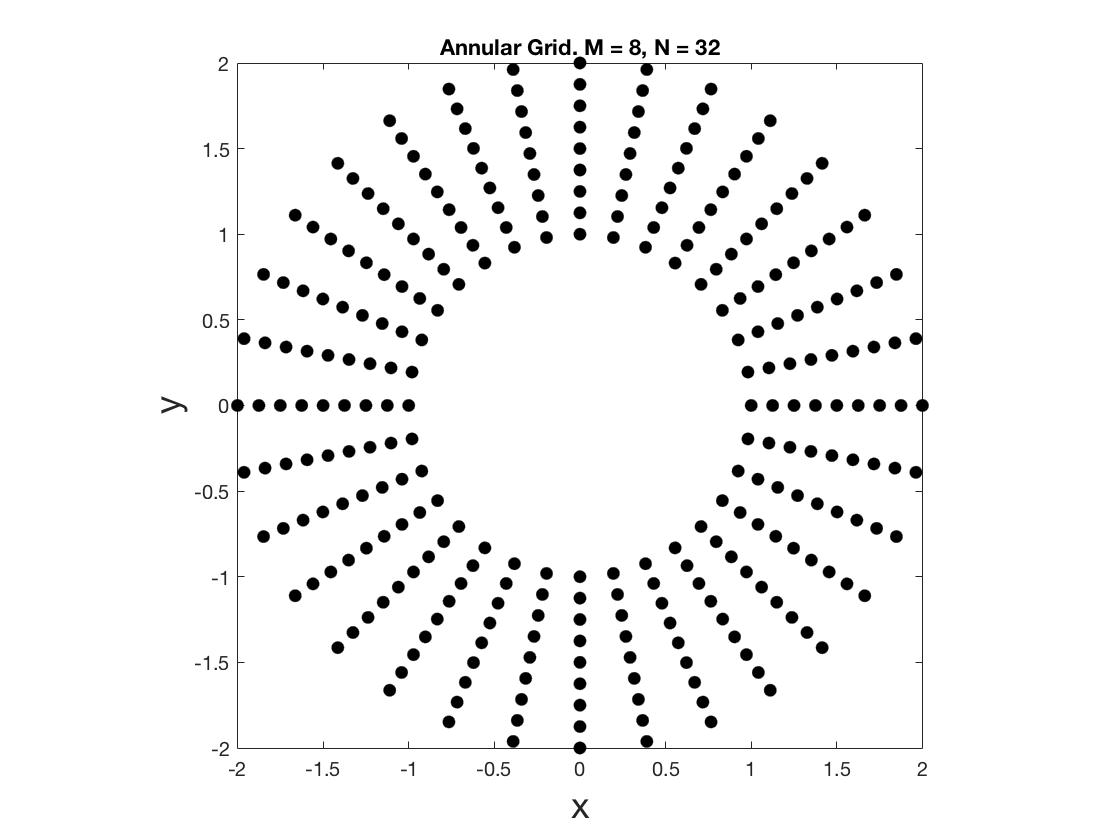
\includegraphics[width= .5\linewidth]{fig_fineGrid.jpg}
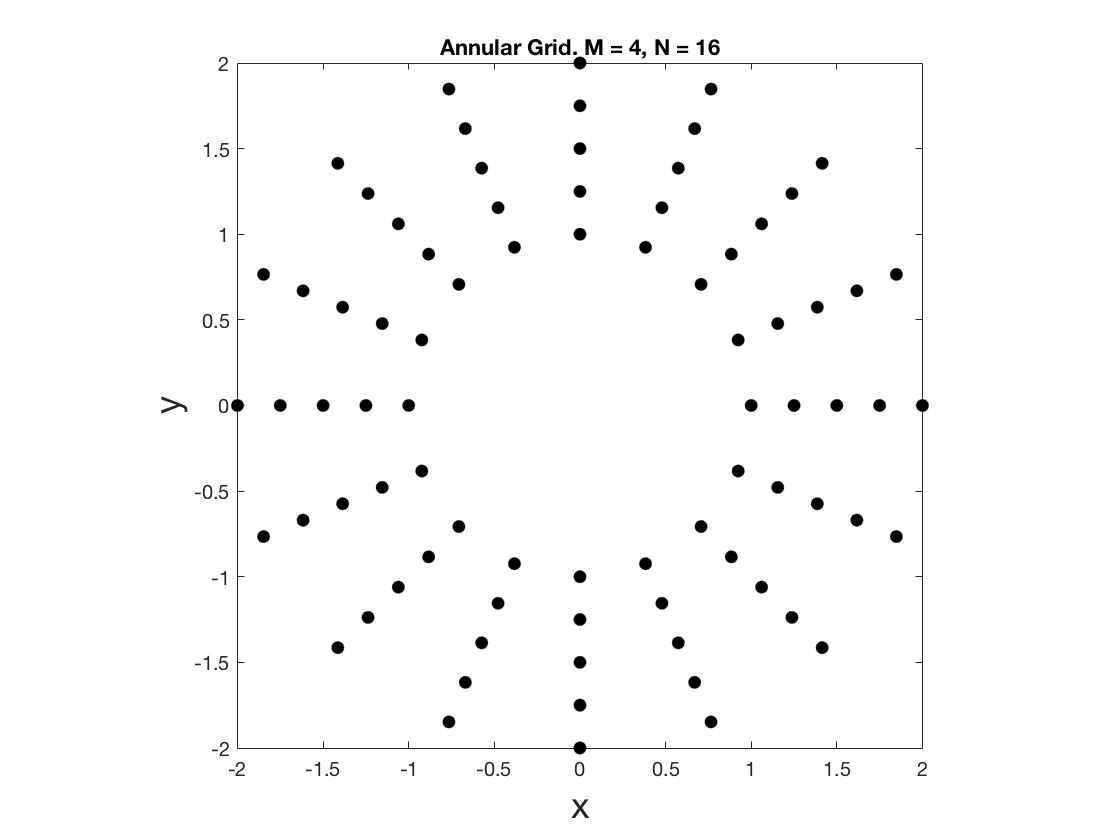
\includegraphics[width= .5\linewidth]{fig_coarseGrid.jpg}
\caption{Discrete points on the Annular Grid for $b=2$. Image on the right has $M$ and $N$ halved compared to the image on the left. }
\label{fig:grid}
\end{figure}

%----------------------------------------------------------------------------------------

\end{column} % End of column 2.2

\end{columns} % End of the split of column 2 - any content after this will now take up 2 columns width

%----------------------------------------------------------------------------------------
%	IMPORTANT RESULT
%----------------------------------------------------------------------------------------

\begin{alertblock}

\begin{figure}
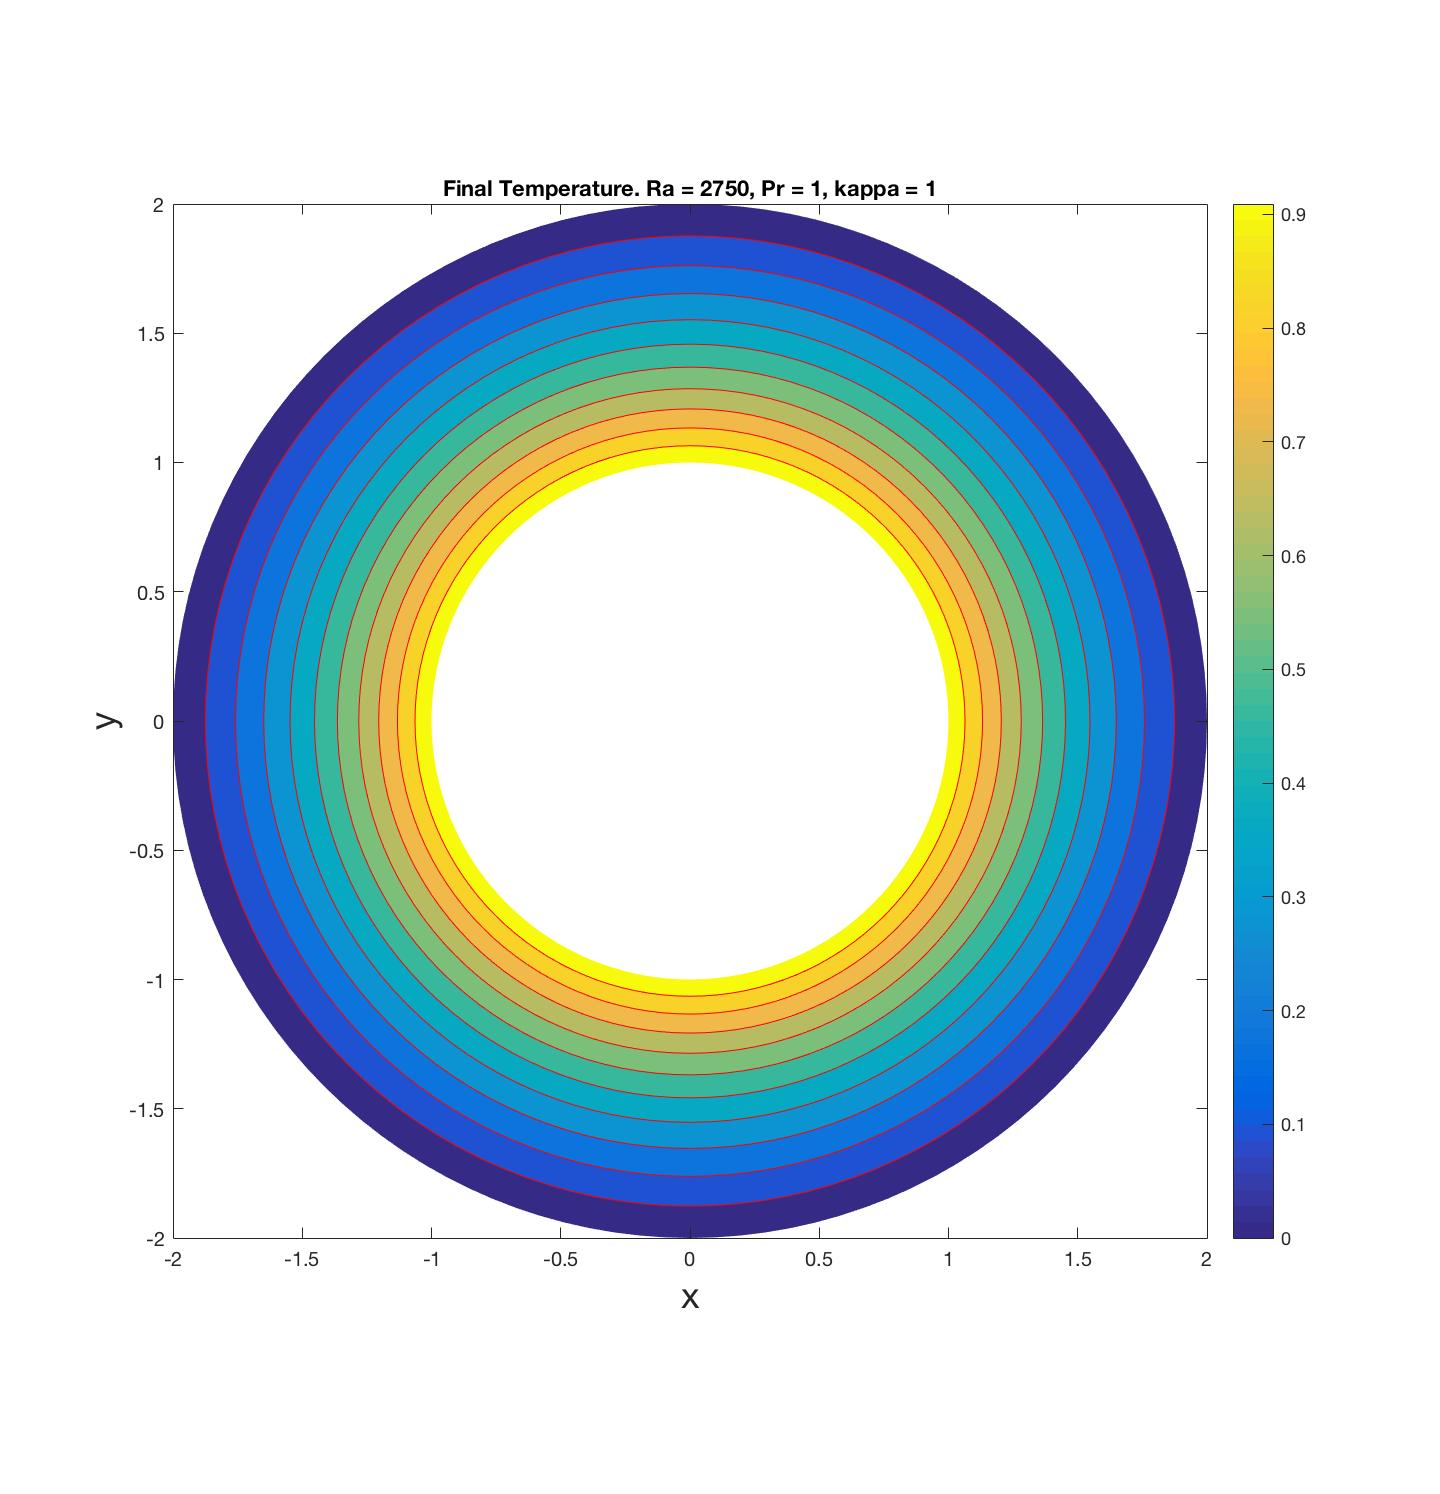
\includegraphics[width= .25\linewidth]{../project_3/fig_q4ra2750}
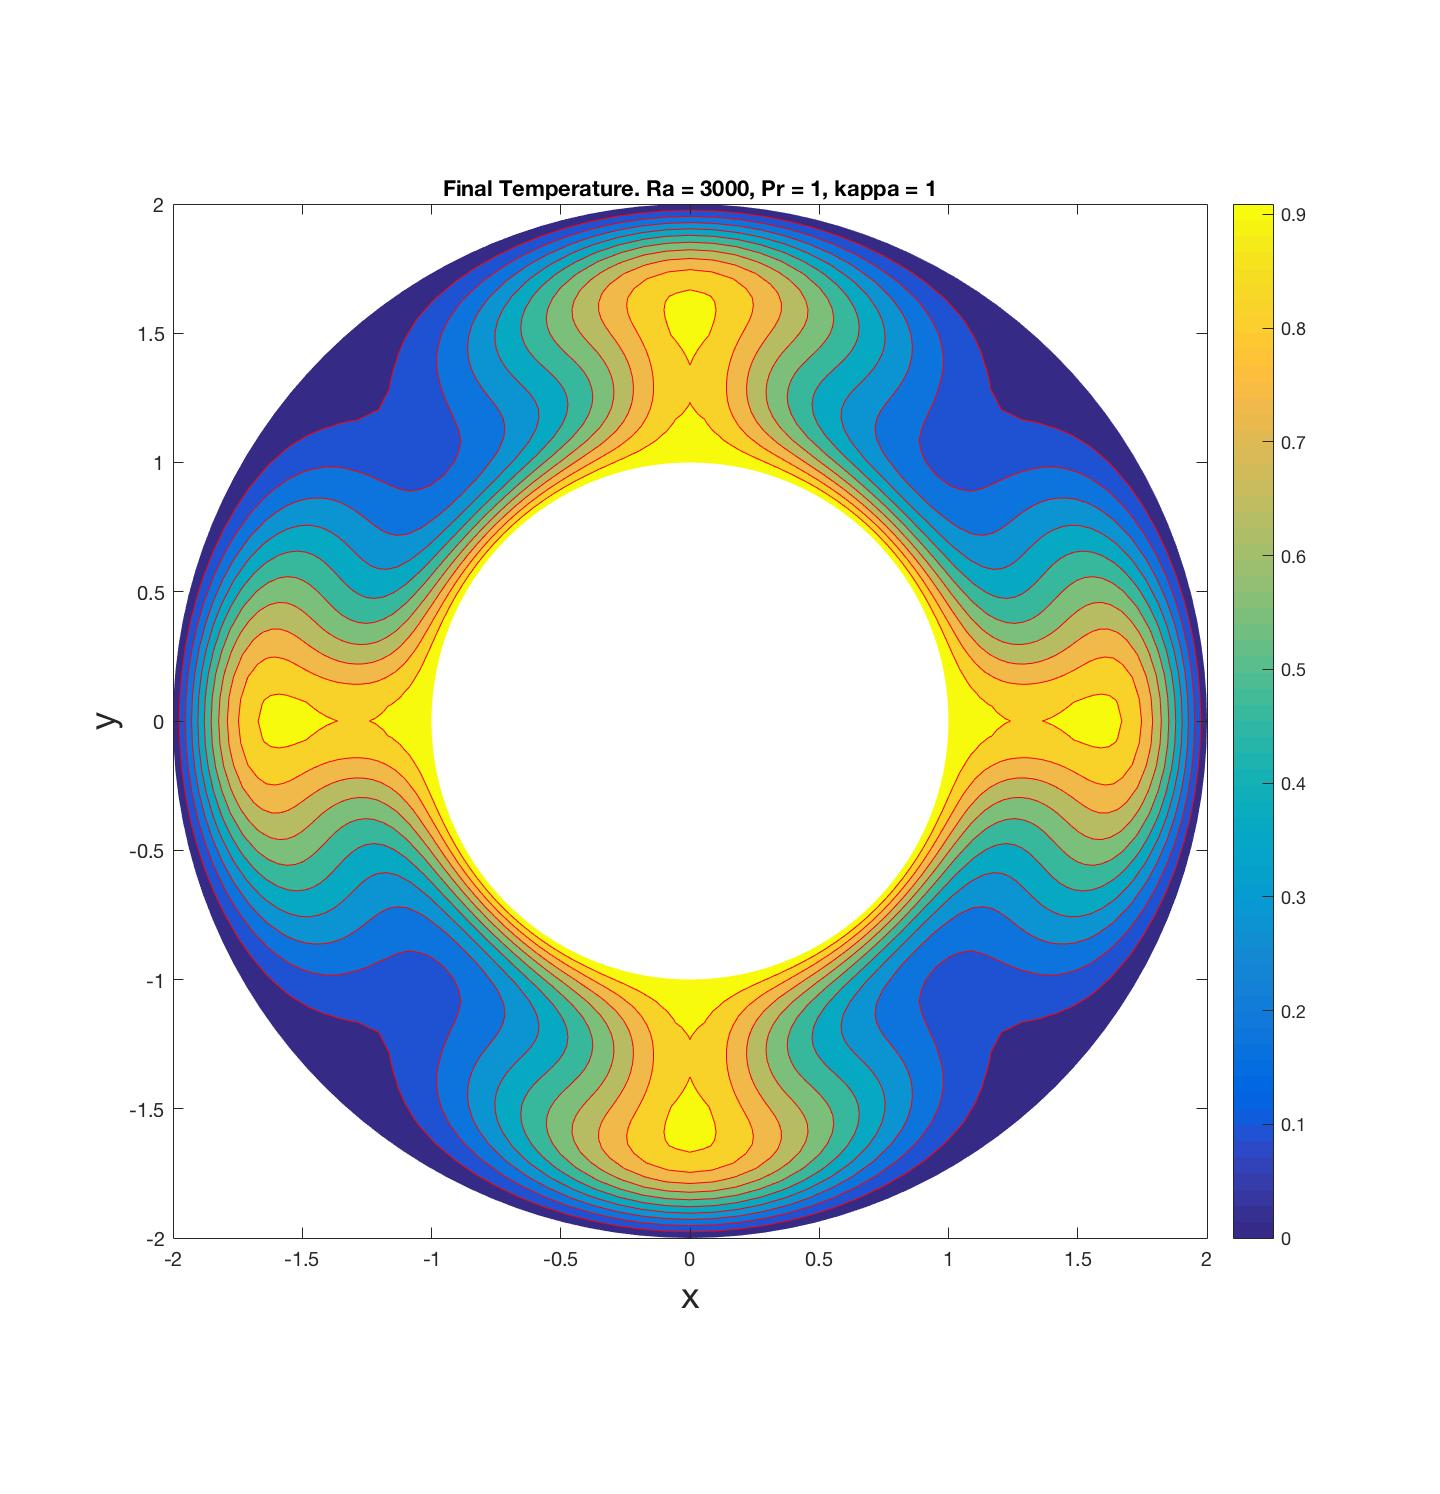
\includegraphics[width= .25\linewidth]{../project_3/fig_q4ra3000.jpg}
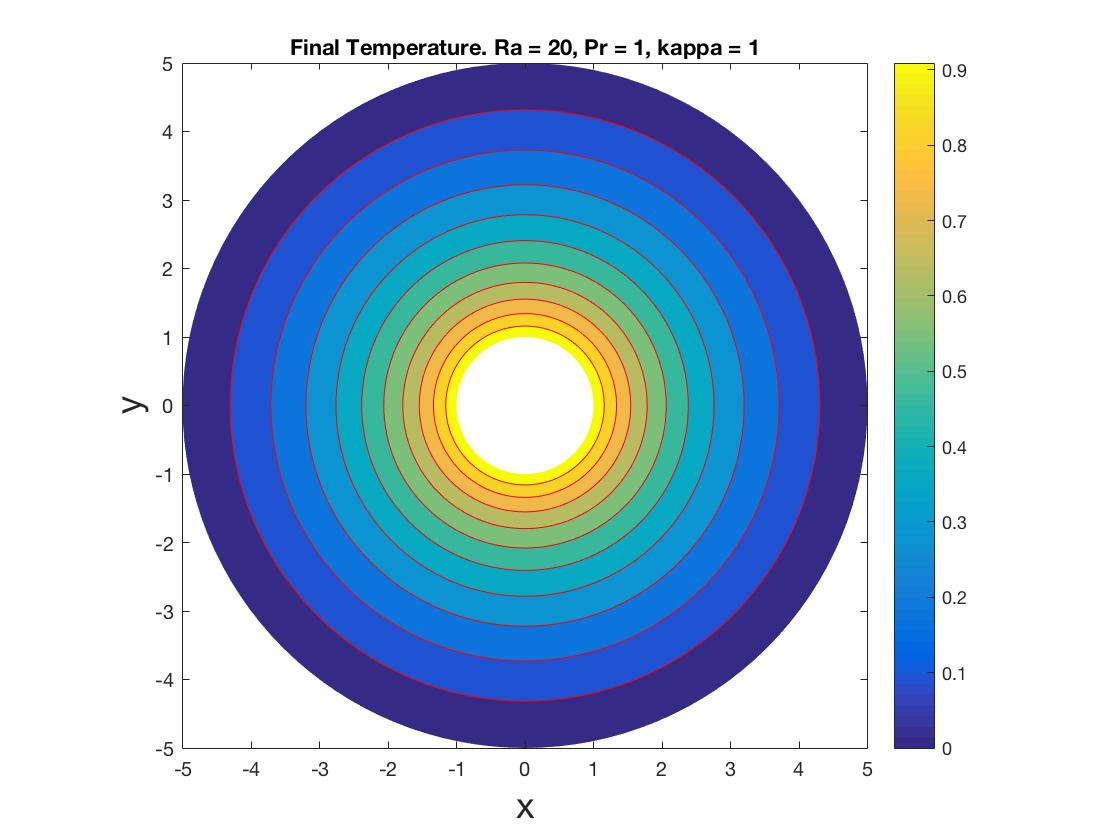
\includegraphics[width= .25\linewidth]{../project_3/fig_q4ra20b5}
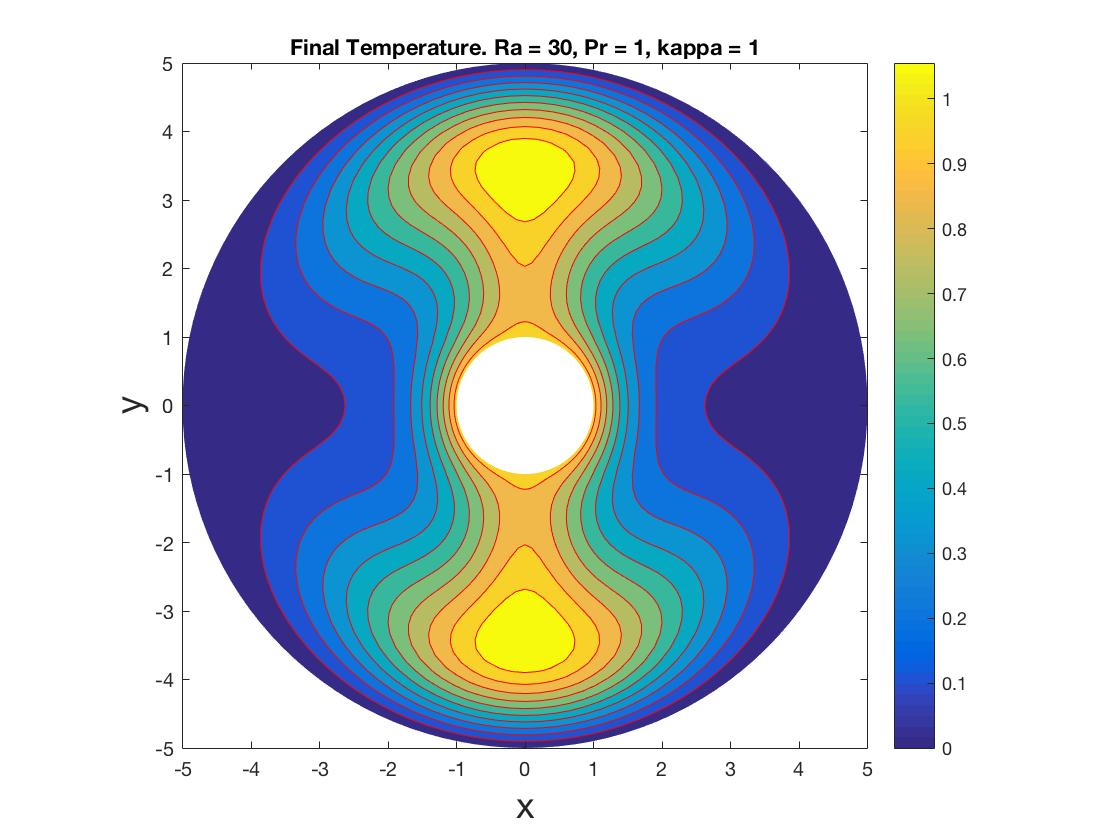
\includegraphics[width= .25\linewidth]{../project_3/fig_q4ra30b5.jpg}
\caption{$\boldsymbol{b=2}$, Left: $R_a = 2750$. Right: $R_a = 3000 \implies R_c \approx 2850$. \\ and $\qquad \boldsymbol{b=5}$, Left: $R_a = 20$. Right: $R_a = 30 \implies R_c \approx 25$. All with $P_r = 1 = \kappa$}
\label{fig:results}
\end{figure}
\end{alertblock} 

%----------------------------------------------------------------------------------------

\begin{columns}[t,totalwidth=\twocolwid] % Split up the two columns wide column again

\begin{column}{\onecolwid} % The first column within column 2 (column 2.1)

%----------------------------------------------------------------------------------------
%	MATHEMATICAL SECTION
%----------------------------------------------------------------------------------------

\begin{block}{Advection-Diffusion Equation}

In order to solve Equation \ref{eq:advectionDiffusion}, an operator splitting approach is taken by first solving for $T_t = - \textbf{u} \cdot \nabla T$ (Advection) and then $T_t = \kappa \nabla^2 T$ (Diffusion) independently.

The Advection part is solved by using a \textbf{Richtmyer's second-order Lax-Wendroff routine} that conserves the scalar field, $T$, being an explicit method. This routine is $\mathcal{O}(\delta r^2,\delta \theta^2,\delta t^2)$ \cite{Mestel}. 

The Diffusion part is solved using an \textbf{implicit Crank-Nicolson scheme}. This done by solving a system of linear of equations ($Ax=b$) using the \textbf{MultiGrid method} that helps compute solutions extremely fast. It does so by accelerating the convergence of an iterative method (\textbf{Gauss-Seidel} in our case) by often computing an approximation on a coarse grid and using it to provide a correction on the finer grid problem.

Figure \ref{fig:kappa} shows the impact of the changing the value of $\kappa$ on the advection-diffusion sub-problem.
\end{block}

%----------------------------------------------------------------------------------------

\end{column} % End of column 2.1
%%%%%%%%%%%%%%%%%%%%%%%%%%%%%%%%%%%%%%%%%%%%%%%%%%%%%%%%%%%%%%%%%%%%%%%%%%%%%%%%
%%%%%%%%%%%%%%%%%%%%%%%%%%%%%%%%%%%%%%%%%%%%%%%%%%%%%%%%%%%%%%%%%%%%%%%%%%%%%%%%
%%%%%%%%%%%%%%%%%%%%%%%%%%%%%%%%%%%%%%%%%%%%%%%%%%%%%%%%%%%%%%%%%%%%%%%%%%%%%%%%
\begin{column}{\onecolwid} % The second column within column 2 (column 2.2)

%----------------------------------------------------------------------------------------
%	RESULTS
%----------------------------------------------------------------------------------------

\begin{block}{Vorticity Equations}

The vorticity equation is 
\begin{align}
	\omega_t + \textbf{u}\cdot \nabla \omega = P_r\nabla^2\omega + P_rF
	\label{eq:omega}
\end{align}
and it is related to the stream function by 
\begin{align}
	-\omega &= \nabla^2\psi
\end{align}

Equation \ref{eq:omega} was again solved using operator splitting by solving $\omega_t + \textbf{u}\cdot \nabla \omega = 0$ (Advection) and then $\omega_t = P_r\nabla^2\omega + P_rF$ (Diffusion) with modified BCs and fundamentally the same schemes as before. $F$ is taken to be $0$ in the full problem. Then $-\omega = \nabla^2\psi$ is solved using a modified MultiGrid solver and \textbf{u} computed using Equations \ref{eq:uPsi}.

\end{block}

\begin{figure}
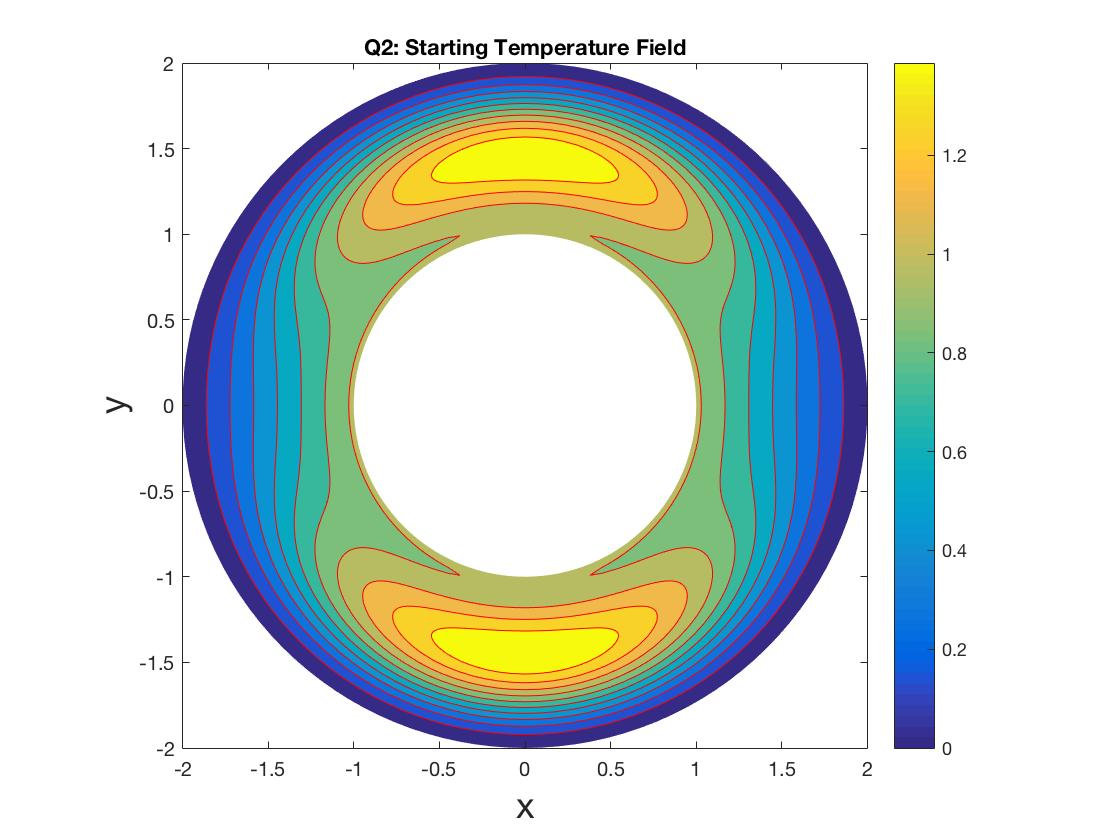
\includegraphics[width= .5\linewidth]{../project_3/fig_q2KappaStart.jpg}
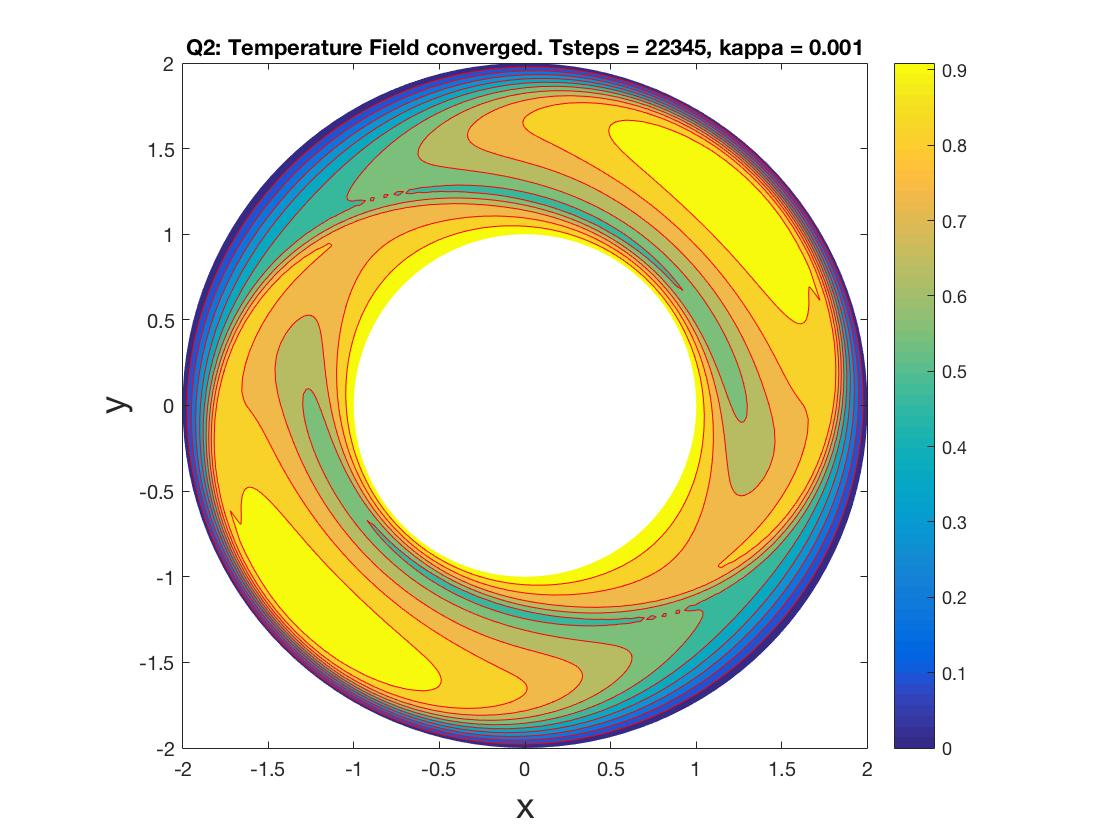
\includegraphics[width= .5\linewidth]{../project_3/fig_q2Kappa0001.jpg}\\
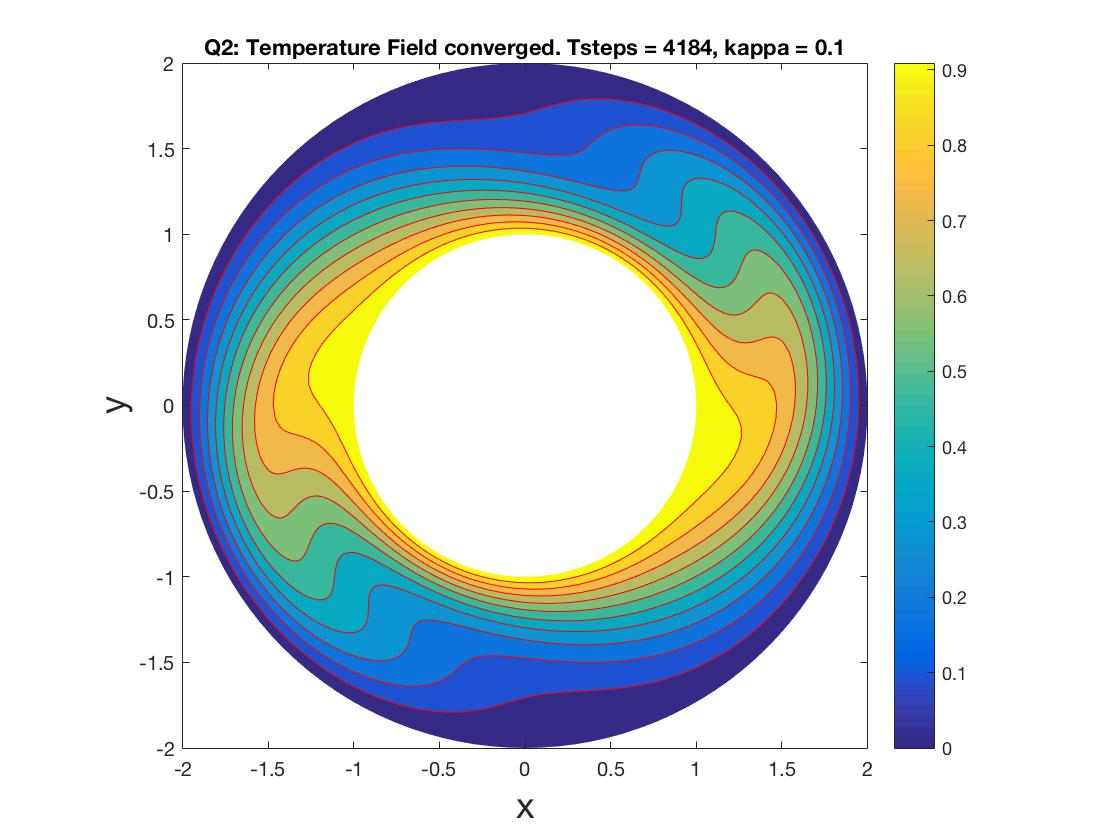
\includegraphics[width= .5\linewidth]{../project_3/fig_q2Kappa01.jpg}
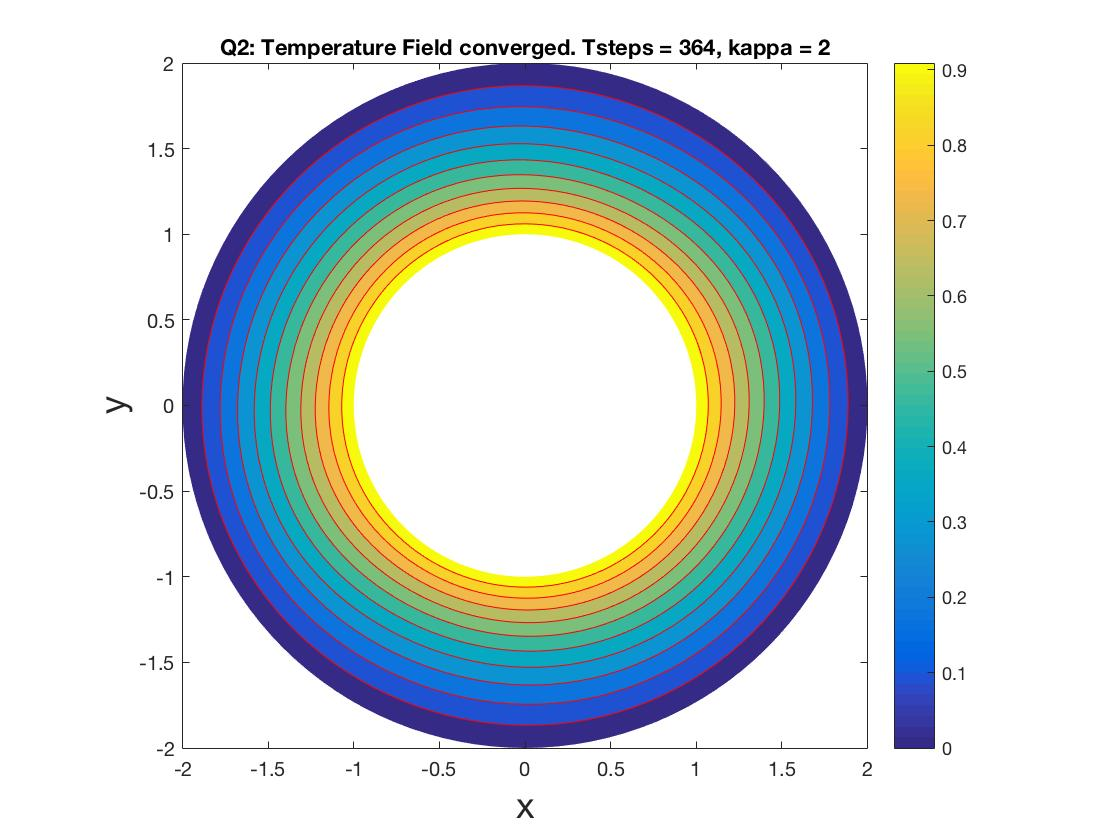
\includegraphics[width= .5\linewidth]{../project_3/fig_q2Kappa2.jpg}
\caption{\footnotesize Top Left: Inital $T$. Top Right: Converged $T$ for $\kappa = 0.001$. BottomLeft: $\kappa = 0.1$. BottomRight: $\kappa = 2$}
\label{fig:kappa}
\end{figure}
%----------------------------------------------------------------------------------------

\end{column} % End of column 2.2

\end{columns} % End of the split of column 2

\end{column} % End of the second column
%%%%%%%%%%%%%%%%%%%%%%%%%%%%%%%%%%%%%%%%%%%%%%%%%%%%%%%%%%%%%%%%%%%%%%%%%%%%%%%%
%%%%%%%%%%%%%%%%%%%%%%%%%%%%%%%%%%%%%%%%%%%%%%%%%%%%%%%%%%%%%%%%%%%%%%%%%%%%%%%%
%%%%%%%%%%%%%%%%%%%%%%%%%%%%%%%%%%%%%%%%%%%%%%%%%%%%%%%%%%%%%%%%%%%%%%%%%%%%%%%
\begin{column}{\sepwid}\end{column} % Empty spacer column

\begin{column}{\onecolwid} % The third column

%----------------------------------------------------------------------------------------
%	CONCLUSION
%----------------------------------------------------------------------------------------

\begin{block}{The Full Problem}
{\small
The full problem is studied by first solving the Advection-Diffusion equations for $T$ and then computing \textbf{u} through the vorticity equations for each time step, and then iterating forward until the solution converges. 

The main focus of the study was initially seeding a $\theta$-dependent perturbation and checking if it grows or decays when varying $R_a$. After a critical value, $R_c$, the behaviour flips. We set $P_r = 1 = \kappa$ and try the compute the value of $R_c$ for various values of $b$ (Figure \ref{fig:results}). Furthermore, for $R_a > R_c$ we studied the behaviour of the rolls that form. As can be seen in Figure \ref{fig:moreResults}, larger values of $R_a$ cause the rolls to be narrower and a larger concentration of high temperature to be near $r=b$. This makes sense as a larger value of $R_a$ simulates a larger thermal driving force.

We also found that not only does $R_c$ varying with $b$ but it also varies upon changing the value of $P_r$. For smaller values of $P_r$, $R_c$ increases. This also makes intuitive sense, as a smaller value of $P_r$ means greater thermal diffusivity which would then require larger thermal driving force to form a convection cell that doesn't diffuse into a linear gradient.
}
\end{block}

\begin{alertblock}

\begin{figure}
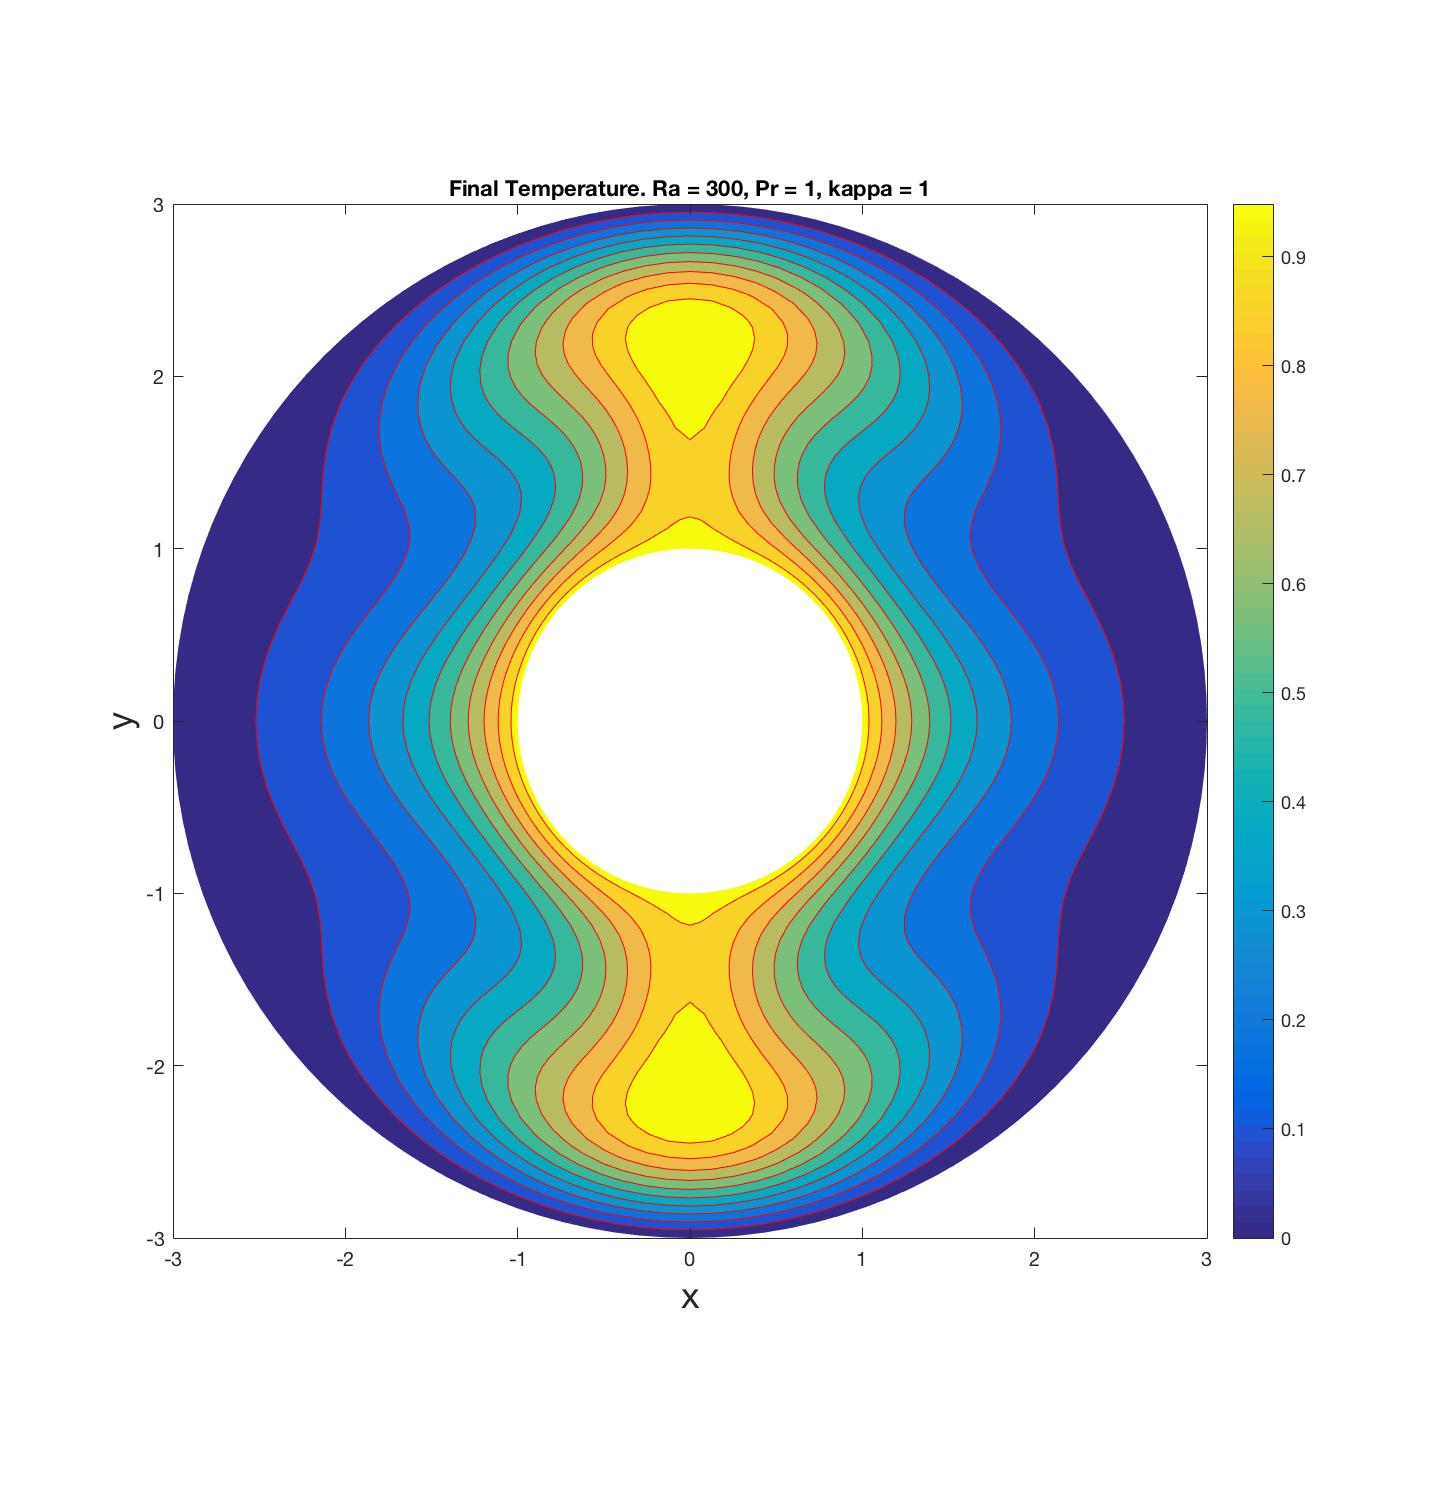
\includegraphics[width= .5\linewidth]{../project_3/fig_q4ra300b3}
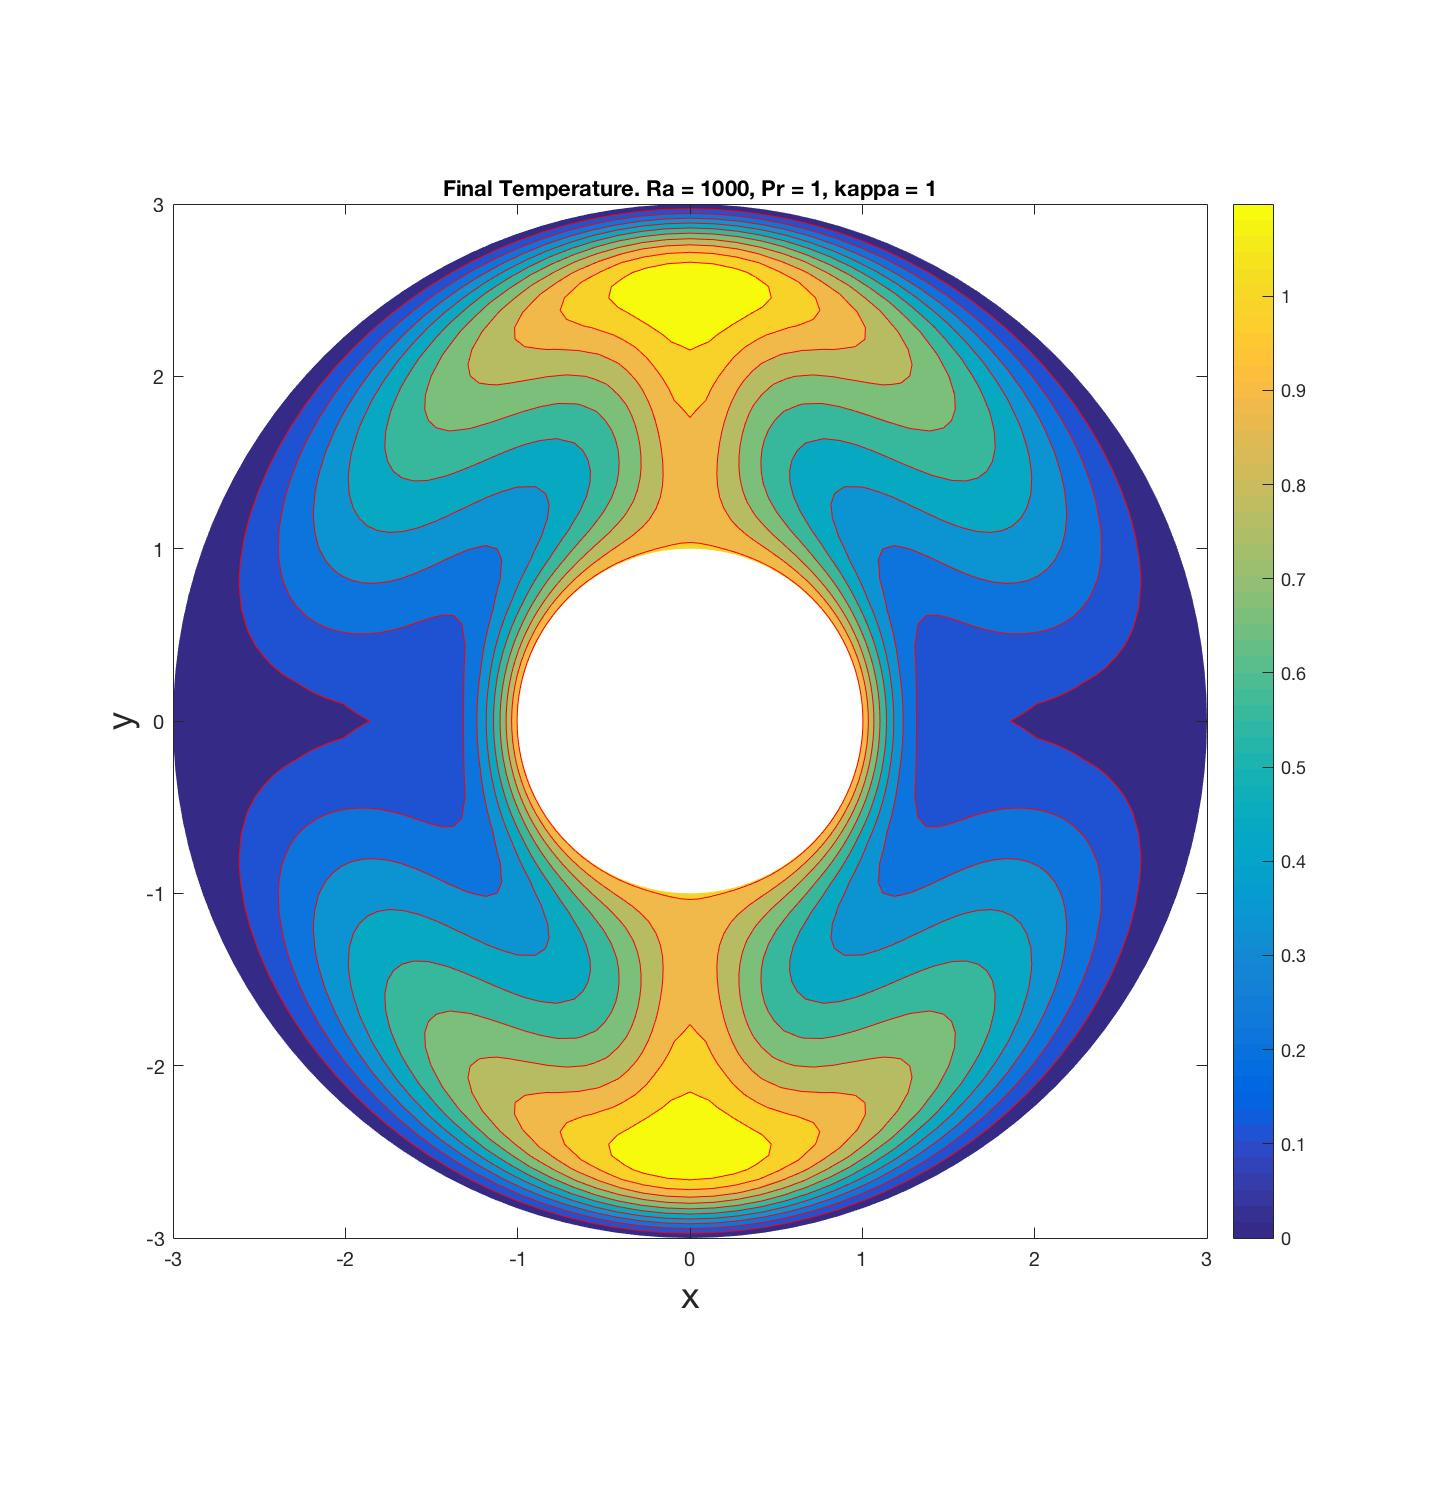
\includegraphics[width= .5\linewidth]{../project_3/fig_q4ra1000b3.jpg}
\caption{$\boldsymbol{b=3}$, Left: $R_a = 300$. Right: $R_a = 1000$. With $P_r = 1 = \kappa$}
\label{fig:moreResults}
\end{figure}
\vspace{-1.5cm}
\end{alertblock} 

%----------------------------------------------------------------------------------------
%	ADDITIONAL INFORMATION
%----------------------------------------------------------------------------------------

\begin{block}{Closing Remarks}

Our implementation of a simplified model of thermal convection in an annulus works as desired. However it depends heavily on the choice of parameters. Although we have studied some of the behaviours within the parameter space, further exploration provides a clear path for future work. 

It is worth noting that many of the results procured are also specific to the initial conditions (the $\theta$-dependent perturbation). Thus studying more scenarios provides another avenue for further research.
\end{block}

%----------------------------------------------------------------------------------------
%	REFERENCES
%----------------------------------------------------------------------------------------

\begin{block}{References}
\nocite{*} % Insert publications even if they are not cited in the poster
\tiny{\bibliographystyle{unsrt}
\bibliography{sample}\vspace{0.75in}}
\end{block}

%----------------------------------------------------------------------------------------

\end{column} % End of the third column

\end{columns} % End of all the columns in the poster

\end{frame} % End of the enclosing frame

\end{document}
